\documentclass[aspectratio=169]{beamer}

\title{Master Thesis Kickoff: Making offline handwriting editable}
\institute{Pattern Recognition Lab (CS~5)}
\date{March 25, 2019}
\author{Martin Stumpf}

\usetheme{fau-tf-lme}

\begin{document}

\maketitle
  
\begin{frame}
  \tableofcontents
\end{frame}

\section{Overview}
\subsection{Introduction}

\begin{frame}{Introduction}
\textbf{"Making offline handwriting editable"}

\begin{itemize}
\item offline vs online handwriting:\\
\begin{columns}
\column{0.27\textwidth}
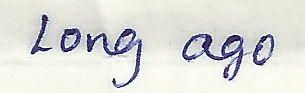
\includegraphics[scale=2.0]{pics/12th-std1-crop.png}
%\hspace{15pt}
\column{0.45\textwidth}
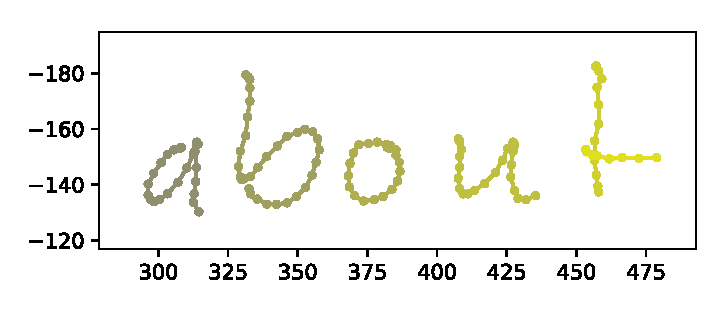
\includegraphics[scale=0.4]{pics/PenPositionsImages.pdf}
\end{columns}\vspace{5pt}
\item 'editable':\\

\includegraphics[scale=1.0]{pics/editable_explanation.pdf}
\end{itemize}
\end{frame}

\subsection{Motivation}
\begin{frame}{Motivation}
\emph{Why?}
\begin{itemize}
\item Combining benefits of digital and handwritten text
\item Automated handwriting generation
\item Because we can (hopefully)
\item Getting new insights into neural networks
\end{itemize}
\end{frame}

\section{Existing Research}
%\subsection{Graves et al.}
\subsection{DeepWriting}
\begin{frame}{Existing Research}
\begin{itemize}
\item \textbf{DeepWriting} by \emph{Aksan et al.}
\item \emph{Conditional Variational Recurrent Neural Network}
\item By design forced to split style and content
\item Can be used to edit the text while keeping the style
\end{itemize}
\begin{center}
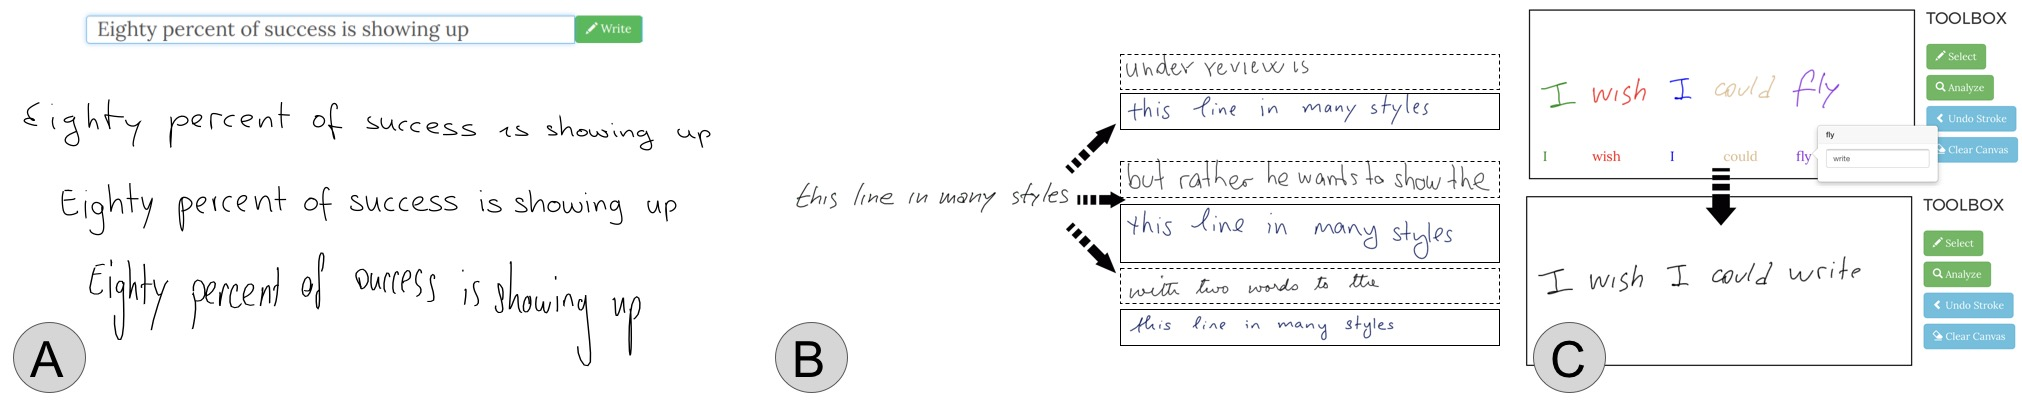
\includegraphics[scale=0.2]{pics/deepWritingExamples.jpg}
\end{center}
\end{frame}

\section{My Approach}
\subsection{Pipeline Overview}
\begin{frame}{Pipeline Overview}
\begin{center}
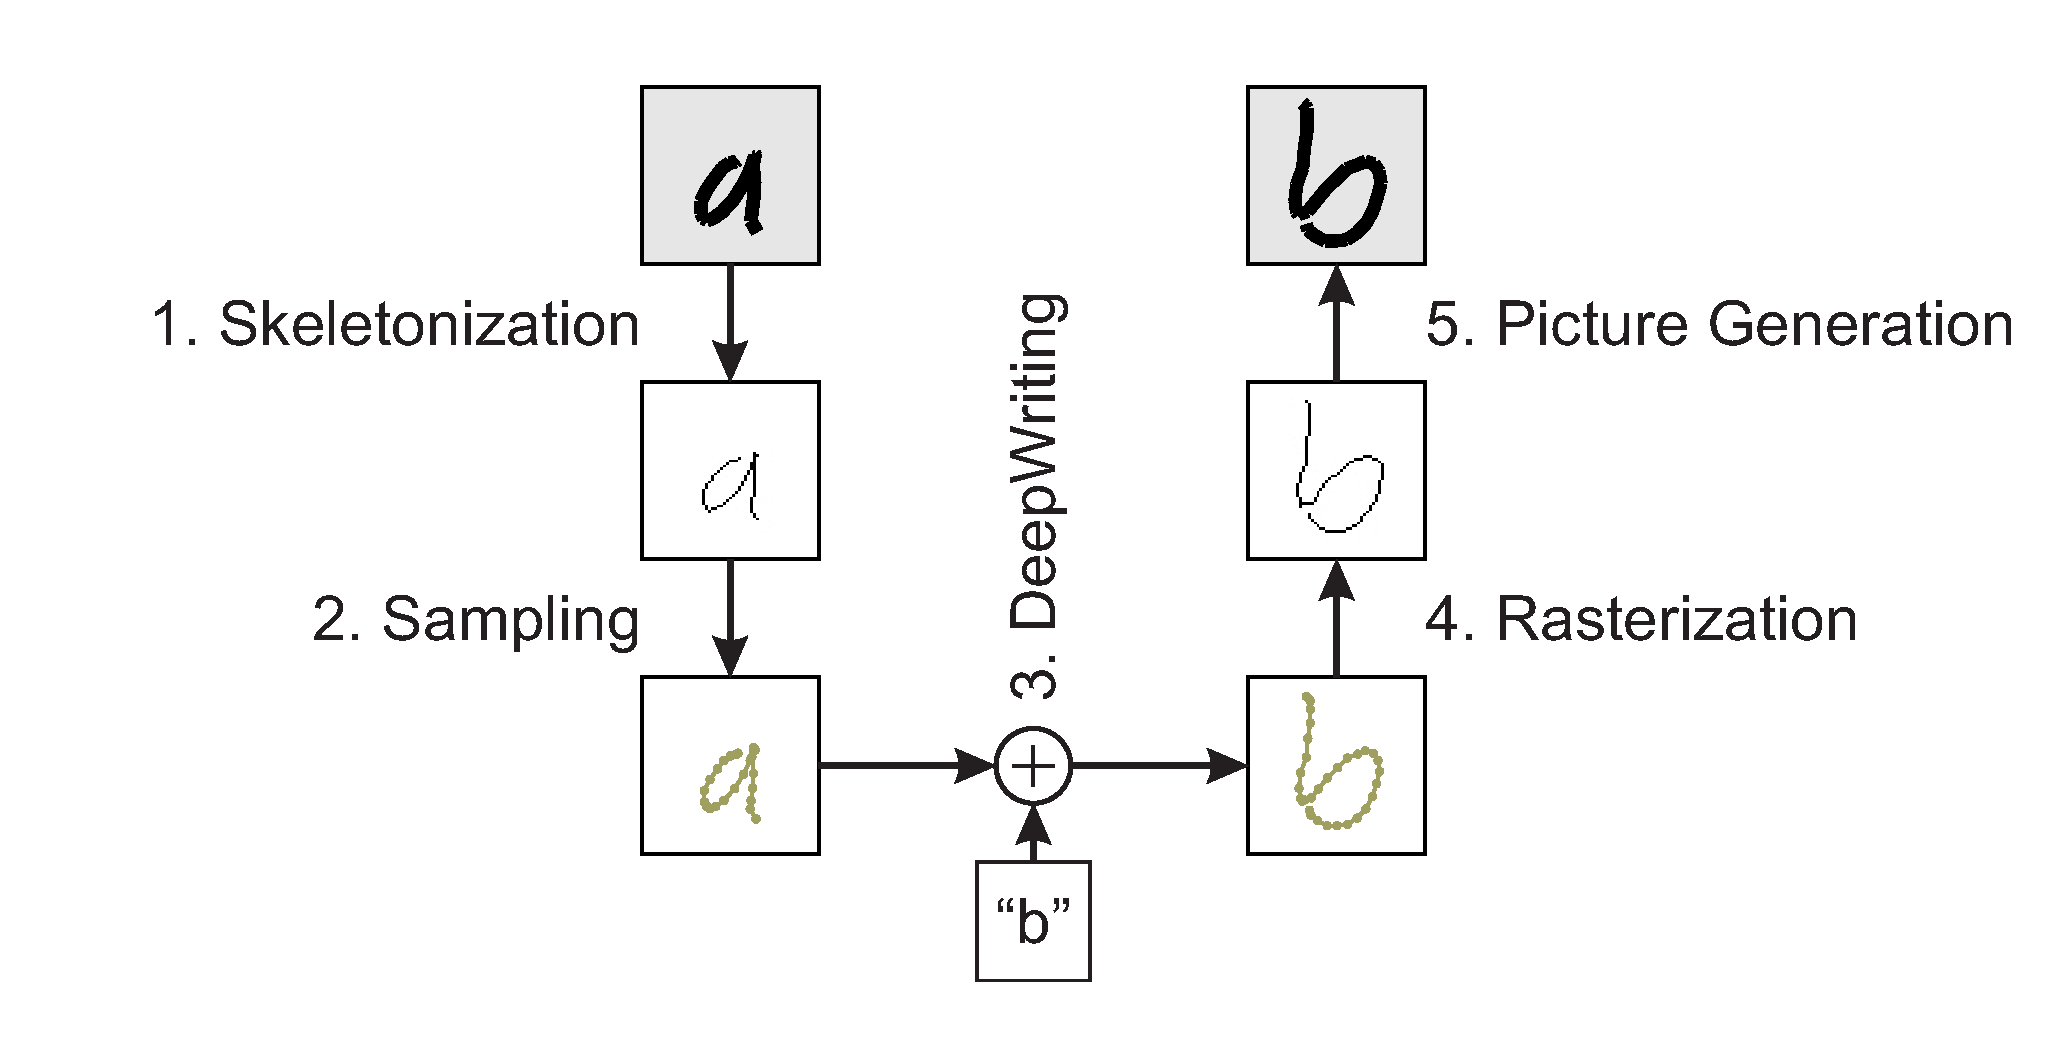
\includegraphics[scale=0.35]{pics/pipeline_numbers.pdf}
\end{center}
\end{frame}

\subsection{Details}

\begin{frame}{Skeletonization}
\begin{itemize}
\item \textbf{Fully Convolutional Network Based Skeletonization for Handwritten Chinese Characters}\\by \emph{Wang et al.}
\end{itemize}
\begin{columns}
\column{0.25\textwidth}
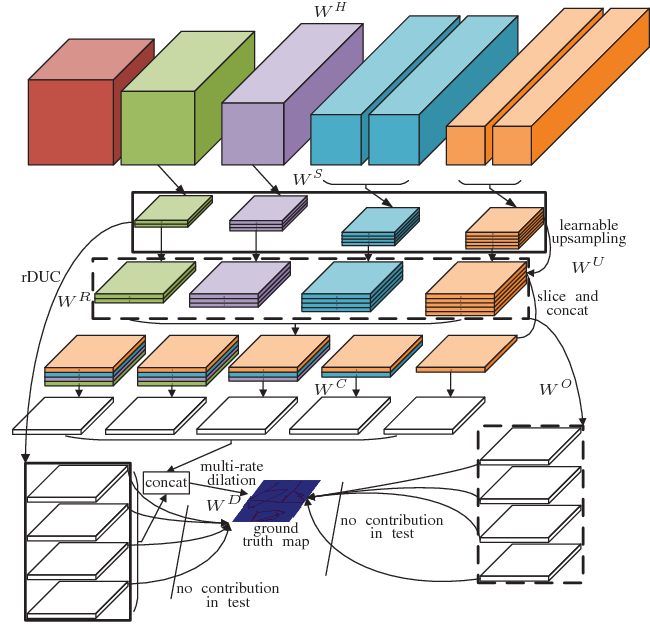
\includegraphics[scale=0.22]{pics/chCharPipe.png}
\column{0.35\textwidth}
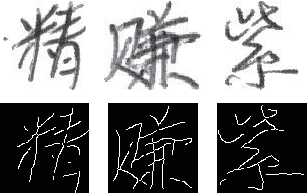
\includegraphics[scale=0.5]{pics/chCharExamples.png}
\end{columns}

\end{frame}

\begin{frame}{Graph Generation and Sampling}
\begin{itemize}
\item heuristic needs to be close enough to human handwriting so DeepWriting understands the underlying structure
\item at the moment the biggest problem
\item current work:
	\begin{itemize}
	\item preprocessing: graph creation, cleanup, merging of crossections
	\item constant distance sampling
	\item reverse engineering the problem
	\item maximum acceleration sampling?
	\end{itemize}
\end{itemize}
\end{frame}

\begin{frame}{DeepWriting and Rasterization}
\begin{itemize}
\item Straight forward, DeepWriting is open source
\end{itemize}
\end{frame}

\begin{frame}{Picture Generation}
\begin{itemize}
\item Conversion of skeleton image to picture
\item \textbf{pix2pix} by \emph{Isola et al.}
\end{itemize}
\begin{center}
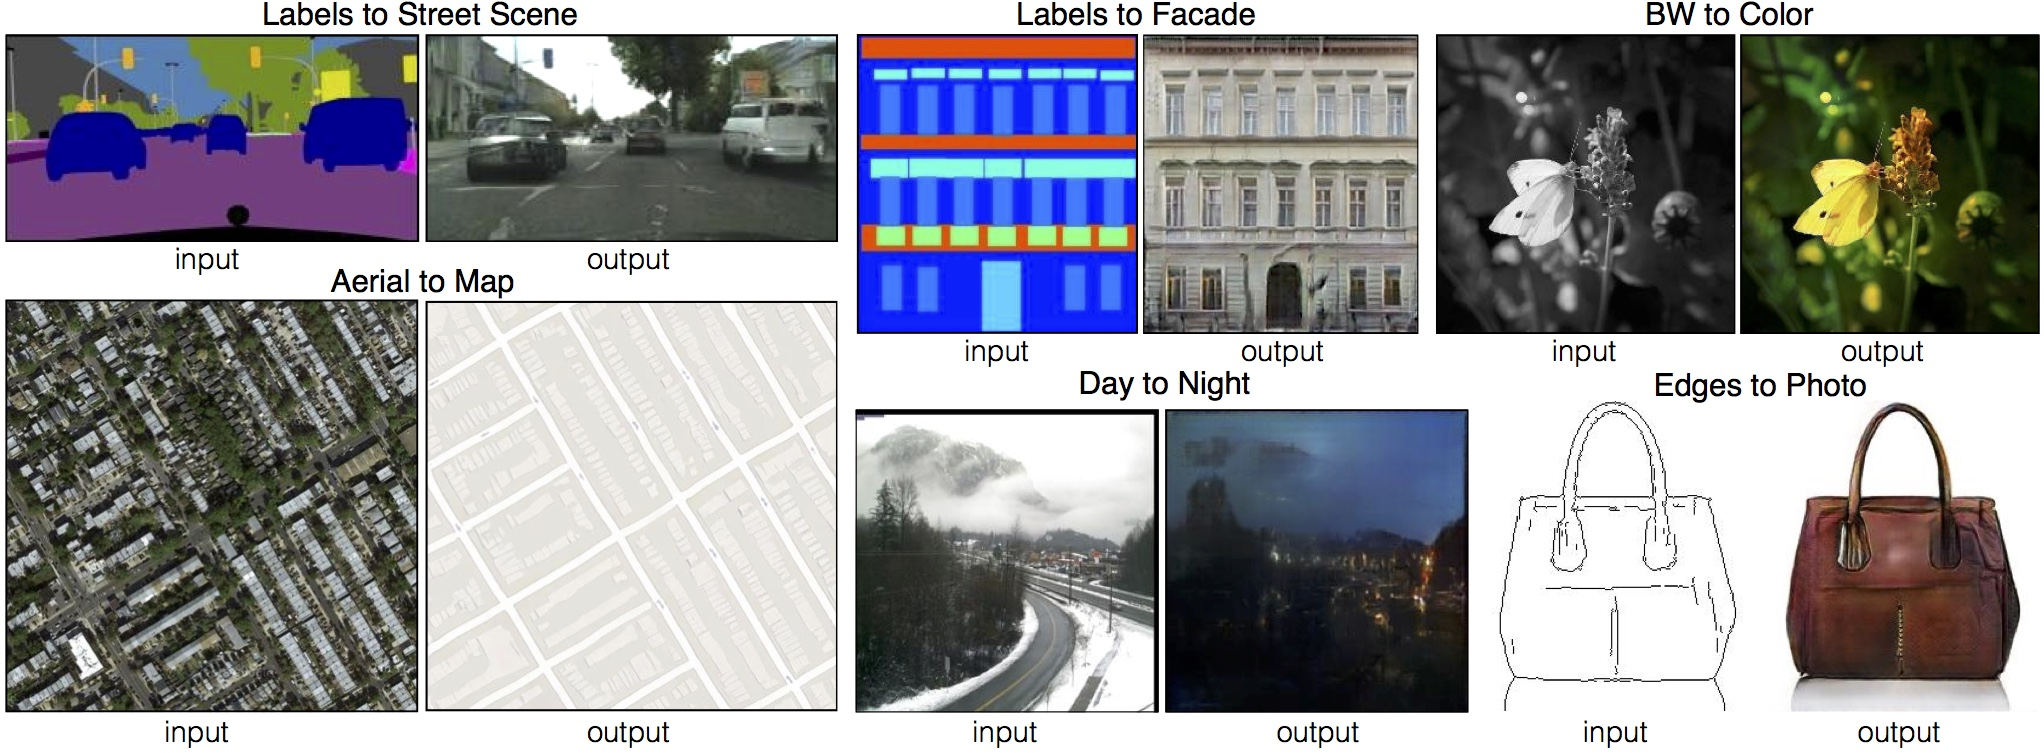
\includegraphics[scale=0.18]{pics/pix2pix.jpg}
\end{center}
\end{frame}

\section{Open Questions}
\begin{frame}{Open Questions}
\begin{itemize}
\item Can DeepWriting be trained on generated samples?
\item Will skeletonization produce usable outputs?
\item Will pix2pix be able to produce believable images?
\item \emph{Future:} How can a visual style transfer be achieved?
\end{itemize}
\vspace{2em}
\begin{center}
\begin{Large}
\emph{Thanks for your attention!}
\end{Large}
\end{center}
\end{frame}



\end{document}
